% !TeX spellcheck = it_IT
\newpage

\section{Paradigmi}
Un \textbf{algoritmo di rendering} è una serie di passi che trasforma la descrizione digitale di una scena e di quattro parametri in un'\textbf{immagine raster}.\\
\begin{figure}[h]
	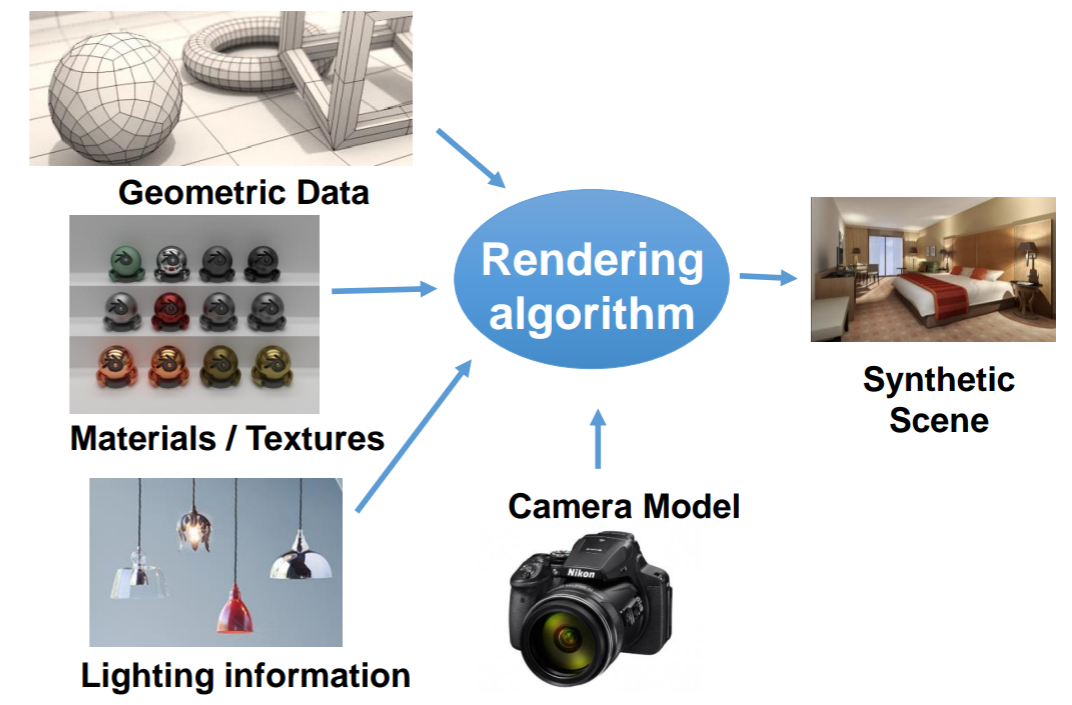
\includegraphics[scale=0.25]{rendering_algorithm.png}
	\centering
\end{figure}

\subsection{Ray Tracing}
L'idea alla base è quella di "sparare" un \textbf{raggio} dal punto di partenza e controllare se ha colpito qualche oggetto.
\begin{lstlisting}[mathescape=true]
	for each pixel p;
		make a ray r (viewpoint to p)
		for each primitive o in scene:
			find intersect(r,o)
		keep the closest intersection $o_j$
		find color of $o_j$ at p
\end{lstlisting}
Non tutti gli oggetti della scena però saranno illuminati, quindi quando un raggio interseca il punto della scena si fa partire un altro raggio che va verso la fonte di luce.\\
Se quest'ultimo incontra un oggetto vuol dire che l'oggetto è in ombra e non è raggiunto dalla luce.\\
C'è da tenere conto che la luce rimbalza un certo numero di volte, tramite il \textbf{reflection ray}. Ovviamente questo costa risorse, più si fa rimbalzare la luce e più l'immagine è realistica e costosa.\\
C'è poi la \textbf{rifrazione} di un oggetto che consiste sempre nel far partire altri raggi una volta che uno raggiunge un oggetto (ad esempio una bottiglia d'acqua).
\subsubsection{Costo}
Dipende da quanti rimbalzi ($N$) facciamo e da quante intersezioni con gli oggetti abbiamo:
\begin{equation}
	RTCost(r)=N \sum_{\forall o \in S} Int(r,o)
\end{equation}
Si noti che $Int(r,o)$ rappresenta il costo dell'intersezione del raggio $r$ con l'oggetto $o$.
\subsubsection{Primitive}
Tutto ciò che riesco facilmente ad intersecare con raggi:
\begin{itemize}
	\item Triangoli, quadrilateri, etc...
	\item Superfici implicite: sfera, geometria solida costruttiva, etc...
\end{itemize}

\subsection{Rasterizzazione}
Nella rasterizzazione (\textit{Transform \& Lighting}) proietto le primitive della scena sul mio schermo, ovvero prendo ogni \textbf{vertice} di ogni primitiva, lo proietto verso il viewpoint e vedo dove interseca la mia finestra. La linea che segna è il \textbf{proiettore}. A partire dalla proiezione dei soli vertici saprò quali pixel selezionare.\\
Il vantaggio principale è che è sufficiente proiettare pochi vertici per rasterizzare gran parte dello schermo.
\begin{lstlisting}
	for each primitive t:
		find where t falls on screen
		rasterize the 2D shape
		for each produced pixel p:
			find the color for t
			color p with it
\end{lstlisting}
\subsubsection{Primitive}
Tutto ciò che so proiettare da 3 dimensioni a 2 e 
\begin{itemize}
	\item Punto
	\item Segmento
	\item Triangolo
\end{itemize}
\subsubsection{Pipeline}
\begin{enumerate}
	\item Identifico le proiezioni delle primitive sullo schermo
	\item Trovo l'area da rasterizzare
	\item La computo
\end{enumerate}
\begin{figure}[h]
	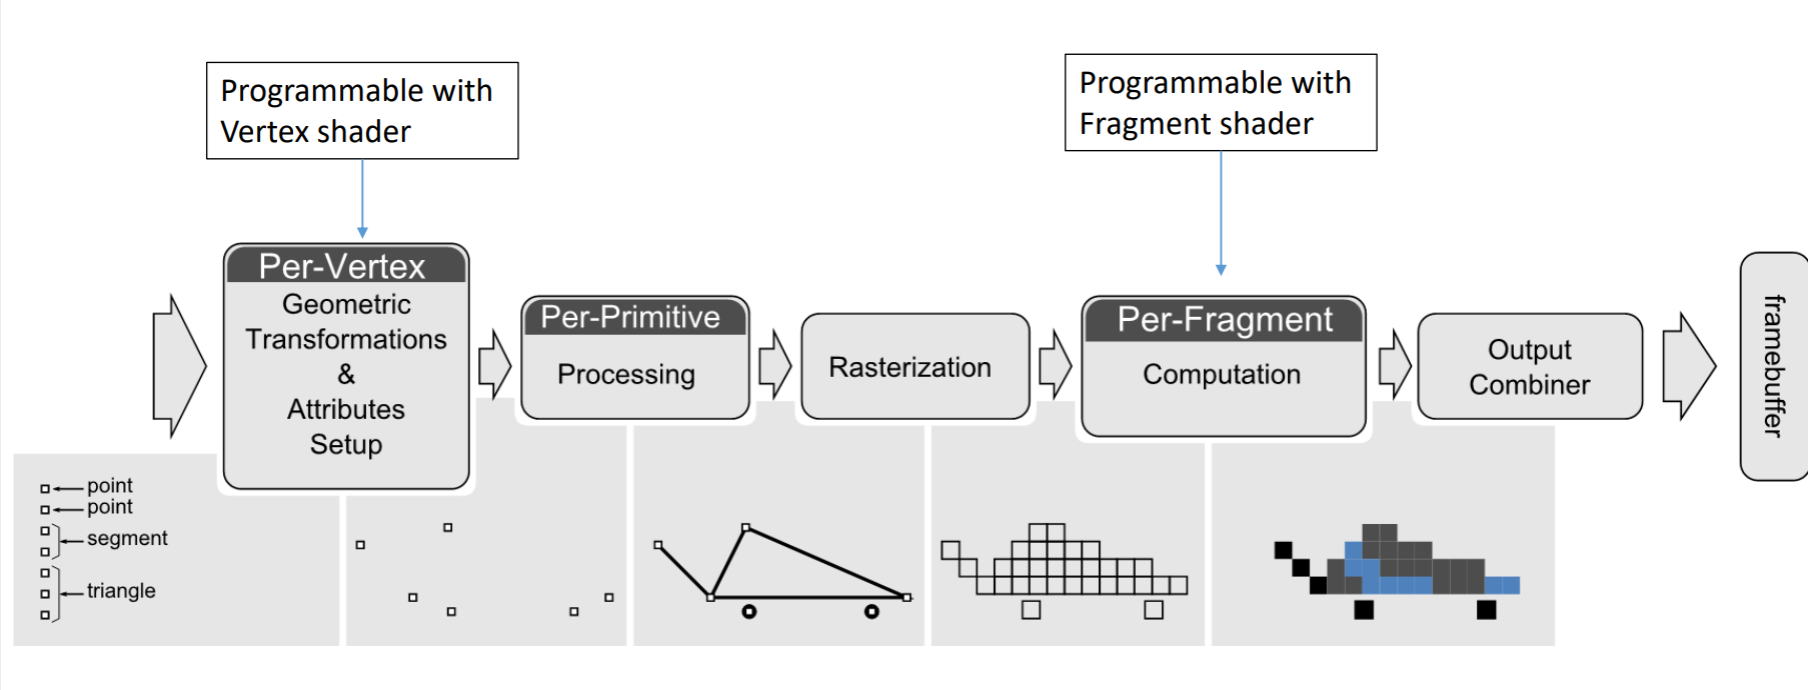
\includegraphics[scale=0.25]{rasterization_pipeline.png}
	\centering
\end{figure}